\documentclass[12pt]{article}
\usepackage[english]{babel}
\usepackage{float}
\usepackage{amsmath}
\usepackage{graphicx}
\usepackage[colorlinks=true, allcolors=blue]{hyperref}

\title{How algorithms help creators}
\author{Dmytro Shapovalov}
\setlength{\parindent}{0pt} % Убирает отступы в начале абзацев

\begin{document}
\maketitle

\section{Introduction}
main source: \cite{0}

\subsection{What are Recommender Systems?}

The internet and modern web services have been growing for the last few decades. An overflow of information is everywhere. It can be challenging for users to surf through all this information to find what they actually need. Many online e-commerce firms recommend products to their users, so they don’t have to search for them by themselves among millions of options. This greatly simplifies finding and purchasing products or services and leads to millions of sales on one platform. With this example we can see how important and useful recommender systems are for both sides—users and companies. Recommender systems aim to solve that information overload problem by personalizing the user list of products or services according to their preferences. More specifically, a recommender system aims to predict if an item would be useful to a user based on given information about the user’s search history and preferences, preferences of other users, and other data. Recommender systems are widely used in e-commerce, retail, streaming services, social media, news, content platforms, and others. High-quality recommender systems positively impact the users’ experience and the overall sales.
\cite{1.1}
\cite{1.2}

\subsection{Creation and improvement}

In 1992, David Goldberg proposed the Tapestry system, the first recommender system based on collaborative filtering through human evaluation. Inspired by these studies, researchers from the Massachusetts Institute of Technology and the University of Minnesota developed the news recommender service, named GroupLens, whose key component is a user-user collaborative filtering model. In 1995, similar recommendation technologies were applied for music by the Ringo system and for video by Video Recommender. Along with the advent of e-commerce, the industry has realized the value of recommendations for business. In the fall of 1997, the GroupLens research lab launched the MovieLens project — a recommender system that asks its users to give movie ratings in order to receive personalized movie recommendations. After that, several MovieLens datasets were continuously released from 1998 to 2019 and became some of the most popular datasets for recommender studies. From the perspective of recommender models, collaborative filtering technologies were the most popular recommender system applications and studies till 2005. Because of the fast development, the community decided to hold the first Recommender Systems Conference in 2007. Currently, ACM RecSys has become one of the most important annual academic conferences that focuses on the study of recommender systems. Since 2016, recommender models based on deep neural networks have emerged in academia and industry. For example, YouTubeDNN (Deep Neural Networks for YouTube Recommenders) was used to improve the accuracy of video recommenders.
\cite{1.3}

\section{How do they work?}
\sloppy
There are several types of recommender systems. Most popular are: Collaborative-Filtering, content based and hybrid based. Each was invented at some point in time, as said in the previous section, and each has its pros and cons. In this section, an explanation of how each of them works is provided.

\subsection{Collaborative filtering}

Collaborative filtering recommender systems rate products by using user's ratings (obvious and not) from historical data. It works by making a database of the users’ preferences for products. And then active users will be compared against this database to detect the active user's neighbours with similar preferences for products. This method relies on the user's historical interactions, such as browsing history, past purchases, or previously listened songs. Collaborative filtering is the commonly used type of recommender system among small companies because it is relatively easy and cheap to develop compared to other types of recommender systems. 
But because of its simplicity, collaborative filtering has several disadvantages, such as the cold-start problem. The term “cold start” originated from automobiles. When the engine is cold, it has problems with starting up, but it has no problems running once it reaches its optimal temperature. The same problem can be applied to recommender systems. When there is a lack of information, a system does not work optimally. Cold starts have two types in this case: product cold starts and user cold starts. Whenever a new product is displayed on an e-commerce site, it goes through the product cold start because there are not enough user interactions with this product, and the system does not know when to display the ad related to that product. The user cold start occurs when a user creates a new account and does not have any product preferences or history of interactions with products to base recommendations on.
\cite{2.1}

\subsection{Content-Based system}

Content based recommender systems attempt to build a user profile to predict ratings on unseen products. It usually uses tags and keywords to calculate ratings. Content-based approaches can be used in many cases where the attribute’s values can easily be extracted. But it’s irrational to use this type of recommender system in cases where attribute values must be manually entered. Content-based approaches do not require other users’ data, as the predicted recommendations only require analyzing the products and individual user profiles. In this way, these techniques allow the system to handle many users. Content based systems are user-independent since this system only requires analyzing the items and user profile for recommendations. 
Opposite of collaborative filtering, content based system does not experience user cold start issues. New products are suggested before a significant list of users appoints a rating. But the content based approach also has several disadvantages, such as product cold start and overload. If not enough information is provided in the content to differentiate products precisely, the recommendation will not work accurately. Also, a content based recommender system can be manageable for small datasets, but when thousands of new products are being added daily, this task is impossible. That is why this type of recommender system is also used only among small companies and cannot be used in large companies with a huge turnover of input data.
\cite{2.2}

\subsection{Hybrid-Based system}

Hybrid based systems combine two or more technologies to achieve better performance. Their main goal is to eliminate the disadvantages of each method. There are several types of hybrid based systems that use different strategies to address the shortcomings of each type of filtering and make the most optimal solution for finding recommendations for users: Weighted, Switching, Mixed, Feature Combination, Cascade, Feature Augmentation, Meta-Level. One of the simplest ones is the weighted hybrid recommender system, which aggregates the results of all combined recommendation approaches and then calculates the recommended item’s score. This approach calculates a linear combination of multiple recommendation scores. However, this model assumes that the relative value (weight) of individual methods is the same for all possible products, which is not always true. The photo below shows the working scheme of such a system:

\begin{figure}[H]  % Начинаем окружение figure для вставки изображения
    \centering     % Центрируем изображение на странице
    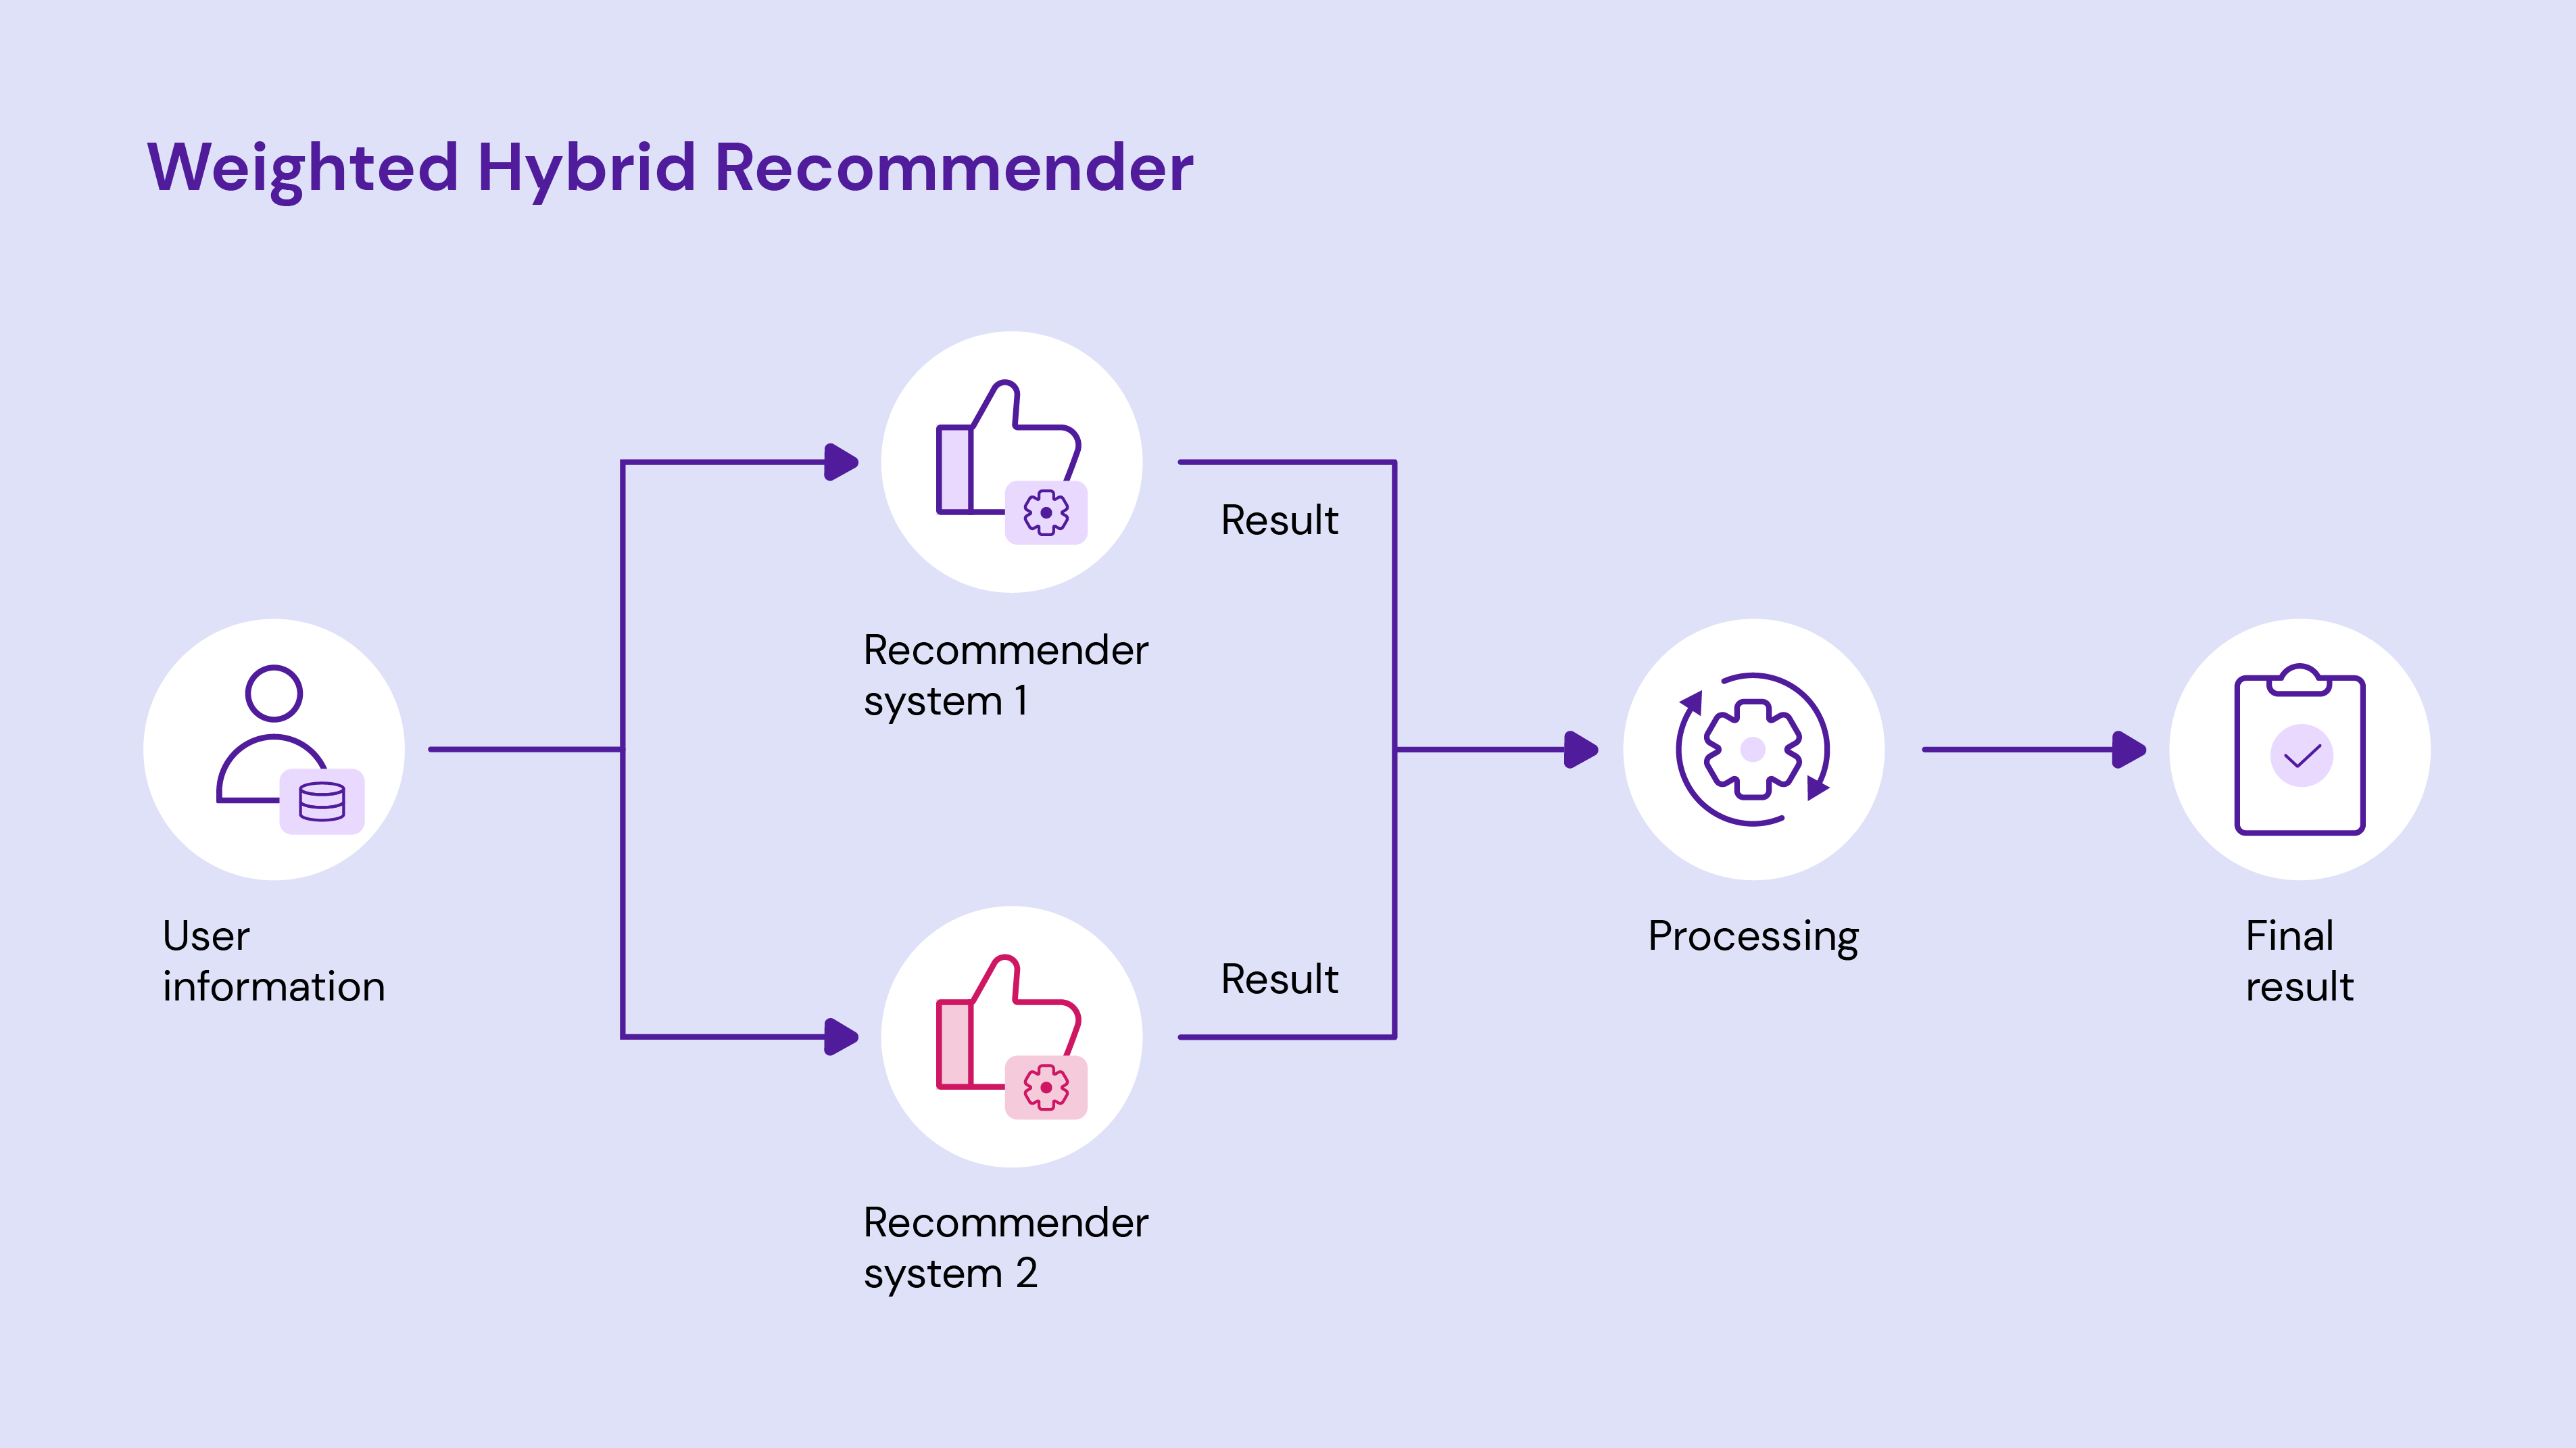
\includegraphics[width=1\textwidth]{image1.png}
\end{figure}
\cite{2.3}
\vspace{1em}

Recommender systems have become a powerful and very important tool for enhancing user experience in various industries in the tech world. Companies use different types of recommender systems depending on their goals. For example, Netflix and Prime Video from Amazon use hybrid models, combining content-based and collaborative filtering systems to recommend their users movies and series that they will like. Amazon and eBay use a content-based recommender system to recommend their products to users. Spotify, Apple Music, and YouTube Music use a content-based recommender system by analyzing track characteristics. YouTube, TikTok, Instagram, and Facebook enhance a combination of hybrid based and deep learning systems. These different types of recommender systems help companies increase engagement and better satisfy the needs of their users.
\cite{2.4}

\section{Real example}

In this section, we will see how recommender systems and their algorithms work on real examples. As examples, I took a social media platform called YouTube. Why YouTube? Because it is a giant in its field with a huge number of active users from all over the world. On its example, it will be possible to see more clearly the power of algorithms in promoting the content of the most different authors.

\subsection{YouTube}

Social media platforms are primarily designed for interaction between users, sharing different types of content (texts, photos, videos), consuming content from other users, and reacting to them by commenting, hitting likes and dislikes, reposting, and others. The most popular examples of such platforms are YouTube, Instagram, TikTok, Snapchat, Twitter (X), and others.
YouTube is the most popular social media platform in the world, owned by Google. It was founded on February 14th, 2005, by Steve Chen, Chad Hurley, and Jawed Karim, three former employees of PayPal. YouTube headquarter is located in San Bruno, California, United States. YouTube is the second-most visited website in the world, after Google Search. In January 2024, YouTube had more than 2.7 billion monthly active users. The rate of videos uploaded to the platform is more than 500 hours per minute, and the total amount is more than 15 billion videos. That's why it's almost impossible for users to find the right video manually.
YouTube employs a sophisticated combination of recommender system types, but mostly it’s a hybrid based system with deep learning. A common misconception is that the YouTube recommender system is there to find an audience for authors' videos, but YouTube explains it differently. The entire purpose of their recommender system is to find the right videos for YouTube’s users, depending on what they and users with similar preferences love to watch.
\cite{3.1}
\subsection{How ordinary users see it}

When a user opens YouTube, he is greeted by a bunch of already-made content. Most likely, most of the offered content will be interesting for him. The YouTube homepage is customized for each user, using algorithms of the recommender system, so that the user wants to dive straight into watching content and using the YouTube application as soon as possible. YouTube collects information about how a user uses the platform, what he has watched previously, how long he watched, what type of content he watched, and other data. 
YouTube's goal is to entice the user to move on to the next video and keep him on the platform for as long as possible. It means that YouTube will offer more and more videos that it assumes the user will like. Also, if a user is not interested in a recommended video, he can click on the “Not interested” button next to the video to help YouTube understand which videos are not worth recommending in the future. Here is a photo of what an ordinary user sees when he starts YouTube:

\begin{figure}[H]  % Начинаем окружение figure для вставки изображения
    \centering     % Центрируем изображение на странице
    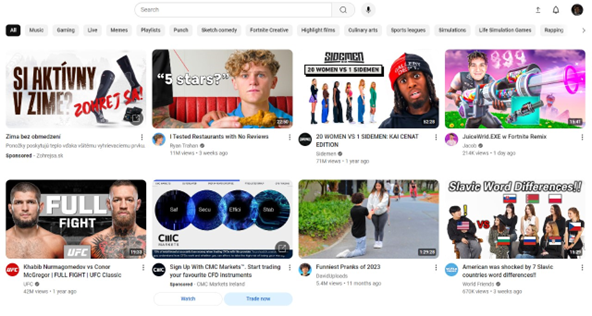
\includegraphics[width=1\textwidth]{image2.png}
\end{figure}

YouTube is ranked as the second most popular search tool in the world after Google and is constantly improving. As stated earlier, its goal is to provide the user with the right information so that he doesn't leave the platform. It goes through each video to find the most relevant to the query based on title, description, tags, and even subtitles. Because of this information, YouTube can better understand what the video is about and figure out if it's a good fit for the user's query. YouTube also takes this information and combines it with data about what content the user has liked in the past before deciding which videos to show in search results.
\cite{3.2}
\section{How authors use recommender systems}

70\% of the watch time is due to the advanced recommendation algorithm. Given that YouTube houses billions of videos, it's vital that the platform recommends the most relevant videos to individual users, otherwise, users will not find videos of interest to them and likely bounce from the platform. These statistics say that YouTube's recommender system is the most powerful tool for authors to gain views, an audience, and, of course, monetization. 
Marketing on YouTube is more than just continually delivering videos and hoping for views, likes, and engagement. Authors need to have a solid understanding of the platform and who uses it, so they know what to create and how to create it. So, here are the main criteria that will increase the chances of a video being seen by algorithms:

\subsection{Front section}

The title and cover of the video give the viewer an idea of what this video is about and help them decide if they want to watch it or not. The cover of the video should be eye-catching. For this purpose, it should stand out from the rest and be bright and unusual. Also, it should convey the main message of the video that users, after they go to the video, remain interested. But its design shouldn't be too difficult to understand. As for the title, there is a similar approach. The title should intrigue users and at the same time be understandable. Put in the title only the most basic words that convey the essence of the video. 

\subsection{Hashtags}

Hashtags increase the visibility of content by categorizing and grouping videos into specific topics or trends. When YouTube users type a specific topic into a search, the platform's algorithm finds videos with those words in the title, description, or tags. If an author includes relevant hashtags in the descriptions, titles, or comment sections of videos, YouTube will match them with viewers' relevant search queries, making these videos easier to find. So, add to the hashtags the most basic and appropriate words for your video, which are most likely to be searched by users. To find out which hashtags are more effective, you can see what hashtags are used in similar videos that are popular.

\subsection{Structure}

The video should be structured in a way that keeps the viewer's attention from beginning to end. Since the more time viewers spend watching video, the better YouTube's recommender system will recommend it to others. Different authors approach it differently. Some videos, such as challenges, are as intense as possible, with exciting events and plot twists every few seconds, and other videos, such as podcasts, on the contrary, attract with their relaxed and simple presentation. But the main thing is to make the viewer watch the video as long as possible.

\subsection{Time}

People tend to watch YouTube at different times of the day, but there are certain peak periods when the number of viewers tends to be higher. The peak is usually in the evenings and weekends when people have more free time. For a better chance of getting recommended, the author should post videos shortly before this period. Here are the statistics of the trending day with respect to view count made by researchers from Tamil Nadu, India:

\begin{figure}[H]  % Начинаем окружение figure для вставки изображения
    \centering     % Центрируем изображение на странице
    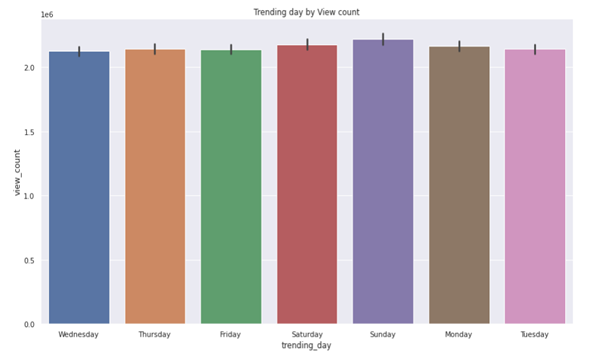
\includegraphics[width=1\textwidth]{image3.png}
\end{figure}
\cite{4.1}
In this graph you can see that the days when users watch content the most are weekends. So, the best time to post videos is on Friday, just before the weekend or right during the weekend, namely on Saturday.

\subsection{YouTube Studio}

With an official app from YouTube called YouTube Studio, creators can monitor watch time, views, and subscriber growth statistics of their channel and individual videos, edit their videos, monetize content and other useful functions that are not available in the main application. This helps them understand what direction to take, what videos to make and what not to make, how to present content to viewers, and much more for better promotion of the channel. Here's a photo of what YouTube Studio looks like:

\begin{figure}[H]  % Начинаем окружение figure для вставки изображения
    \centering     % Центрируем изображение на странице
    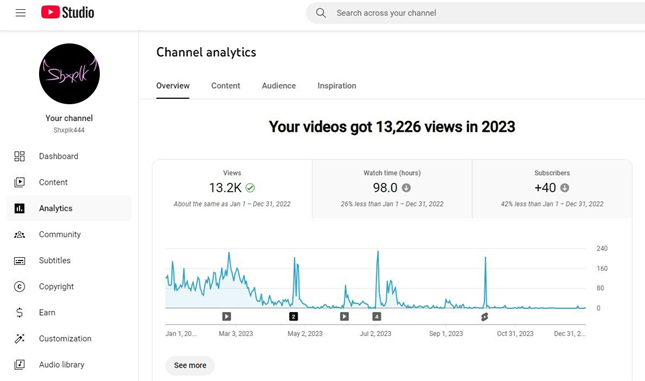
\includegraphics[width=1\textwidth]{image4.png}
\end{figure}

\cite{4.2}

\section{Problems of recommender systems}

The invention of recommender systems has made the work of content creators easier and helped in the promotion of large companies. But not everything is as perfect as we would like it to be. Recommender systems have their own disadvantages. In this section, the main ones are provided. 

\subsection{User privacy}

User privacy is one of the biggest problems for recommender systems because a majority of the most successful recommender systems are based on hybrid based or collaborative filtering systems, which work by constructing models of their users to generate personalized recommendations that are different for each user. That is why using user data is unavoidable. Privacy risks may occur when data are collected or shared without the user’s explicit agreement. Also, once data sets are stored, there is the additional risk that data may be leaked or become subject to deanonymization attempts. In both cases, privacy violations expose users and their private information to risks. 
Currently, there are 3 main types of solutions to these problems: architectural, algorithmic, and political. The architectural solution aims to minimize risks of privacy leakage by storing user data in separate and decentralized database sets. The algorithmic solution aims to minimize the risk that user data could be exploited by using encryption on this data. Political approaches introduce sanctions to regulate the collection, usage, and storage of data. Also, in 2017 Dimitris Paraschakis proposed a user-centered recommendation framework, letting users decide whether their data can be shared or not and with whom. But however user-centered approaches have limits, as they may be just a reassignment of responsibility.
\cite{5.1}

\subsection{Prejudgment towards new content}

This problem is more relevant for content authors. Recommender systems' algorithms often rely on content that has already gained an audience. As a result, already popular channels continue to gain views and popularity, while it becomes harder for new ones to carry forward their content. This creates a bias in audience reach towards channels with experience and can demotivate creators whose content doesn't fit into popular trends.

\section{Conclusion}

Recommender systems have made their input to the world of technology. Their algorithms simplify the lives of ordinary users around the world by providing quick access to trending and interesting content for them. Millions of people all over the world who like to watch TikTok feed, reels on Instagram, or just new videos on YouTube can't imagine life without recommendations and their algorithms, even though they may not know what they are and how they work. For authors, recommender systems became a powerful tool for promoting their content, expanding their reach, and finding their target audience. Large companies such as YouTube, TikTok, Instagram, and others use recommender systems to encourage new users to start using their service and not new ones to continue. In this way, recommendations have become an essential part of today's Internet space, affecting all sides—users, content creators, and companies.

\bibliographystyle{unsrt}
\bibliography{sample}

\end{document}